\documentclass[10pt]{beamer}
\usetheme{Frankfurt}
\usecolortheme{dolphin}
\usepackage[utf8]{inputenc}
\usepackage[spanish]{babel}
\usepackage{amsmath}
\usepackage{amsfonts}
\usepackage{amssymb}
\usepackage{graphicx}
\usepackage{ragged2e}
\setbeamertemplate{navigation symbols}{} 
\author[Kevin García - Alejandro Vargas]{Kevin García 1533173 \newline Alejandro Vargas 1525953}
\institute{Universidad del Valle}
\title{Diseño y validación de muestreo de cítricos para detección de enfermedades en viveros del Valle del Cauca}

\newcommand\Wider[2][3em]{%
\makebox[\linewidth][c]{%
  \begin{minipage}{\dimexpr\textwidth+#1\relax}
  \raggedright#2
  \end{minipage}%
  }%
}
%\setbeamercovered{transparent} 
%\setbeamertemplate{navigation symbols}{} 
%\logo{} 
%\institute{} 
%\date{} 
%\subject{} 
\begin{document}
\begin{frame}[plain]
\maketitle
\end{frame}

\begin{frame}{Contenido}
\tableofcontents
\end{frame}

\section{Proyecto}
\begin{frame}
\frametitle{Información del proyecto}
\begin{block}{Entidad encargada}
\begin{itemize}
\justifying
\item AGROSAVIA (Corpoica)
~\\La Corporación Colombiana de Investigación Agropecuaria, Corpoica, es una entidad pública descentralizada de participación mixta sin ánimo de lucro, de carácter científico y técnico, cuyo objeto es desarrollar y ejecutar actividades de Investigación, Tecnología y transferir procesos de Innovación tecnológica al sector agropecuario.
\end{itemize}
\end{block}
\begin{block}{Personal a cargo}
\begin{itemize}
\item[-]Nubia Murcia Riaño (Investigador Ph.D.)
\item[-]Mauricio Fernando Martínez (Investigador Máster)
\item[-]Elizabeth Narvaez Toro (Líder de Seguimiento y Evaluación)
\end{itemize}
\end{block}
\end{frame}

\section{Problema}
\subsection{Problema contextual}
\subsection{Problema estadístico}
\begin{frame}
\begin{block}{Problema contextual}
\justifying
~\\Existen diversas enfermedades en los cítricos transmitidas principalmente por injertación, vectores (organismos o insectos), y uso de herramienta, las cuales son muy dañinas para este cultivo, entre ellas, el virus de la tristeza, HLB, Leprosis y Exocortis. Estas debilitan el árbol, generando producciones escasas, y en casos avanzados puede llegar a matar el árbol. El inconveniente es que estas enfermedades son asintomáticas en edades tempranas de la planta, es decir, no podemos diferenciar a simple vista una planta infectada con una no infectada. Al sembrar una planta con alguna de estas infecciones desde el comienzo, se perderá mucho dinero invirtiendo en su mantenimiento, por lo cuál se necesita asegurar o garantizar que las plantas que van a ser sembradas y entregadas estén limpias de estas enfermedades, logrando de esta manera la producción de material certificado.
\end{block}
\begin{block}{Problema estadístico}
\begin{itemize}
\justifying
\item ¿Es posible diseñar un plan de muestreo adecuado y asequible que permita la detección temprana de estas enfermedades en los cítricos?
\end{itemize}
\end{block}
\end{frame}


\section{Justificación}
\begin{frame}
\frametitle{Justificación}
\justifying
Nuestro rol como estadísticos es de vital importancia para lograr verificar que la producción esté libre de cualquier plaga y mitigar en gran medida posibles pérdidas en toda la industria por lotes infectados, logrando que productores y consumidores se ven beneficiados.
\end{frame}

\section{Objetivos}
\subsection{Objetivos general}
\subsection{Objetivos específicos}
\begin{frame}
\frametitle{Objetivos propuestos}
\begin{block}{Objetivo general}
Diseñar y validar un plan de muestreo para aceptación y rechazo de lotes de cítricos en viveros del Valle del Cauca que permita estimar la cantidad de plantas infectadas en el lote.
\end{block}
\begin{block}{Objetivos específicos}
\begin{itemize}
\justifying
\item[-]Proponer y diseñar diferentes tipos de muestreo tipo aceptación/rechazo para lotes de cítricos en viveros del Valle del Cauca.
\item[-]Validar los diseños muéstrales por medio de simulación teniendo en cuenta confianza y costo del muestreo.
\item[-]Estimar la cantidad de plantas infectadas en el lote.
\end{itemize}
\end{block}
\end{frame}

\section{Variable de interés}
\begin{frame}
\frametitle{Variable de interés}
~\\Nuestra variable de interés se puede definir de la siguiente manera:
$$X= \left\{\begin{array}{cc}
             1 &   si \; la \; planta \; esta \; infectada \\
             \\ 0 &  si \; la \; planta \; no \; esta \; infectada \\
             \end{array}
   \right.$$
\end{frame}


\begin{frame}
\frametitle{Variable de interés}
~\\Para llegar a la variable de interés definida anteriormente, se lleva a cabo una prueba de laboratorio en la cuál se pueden medir hasta 45 muestras de tejido de plantas, donde se obtiene al final una coloración en el recipiente, a esta coloración se le hace una lectura visual o colorimétrica, usualmente se utiliza más la medida colorimétrica por ser mas objetiva, esta se obtiene con un valor de absorbancia, que corresponde en pocas palabras a una cuantificación de la percepción del color. Se encuentra de la siguiente manera:
\[ A_\lambda=-log_{10} \left( \frac{I}{I_0}\right) \]
~\\Donde:
~\\I es la intensidad de la luz con una longitud de onda específica $\lambda$ tras haber atravesado una muestra (intensidad de la luz transmitida).
~\\$I_0$  es la intensidad de la luz antes de entrar a la muestra (intensidad de la luz incidente).
\end{frame}

\section{Antecedentes}
\subsection{Antecedentes contextuales}
\begin{frame}
\frametitle{Antecedentes}
\begin{block}{Antecedentes contextuales}
\begin{itemize}
\justifying
\item[1.]Epidemiología de Plum pox virus y citrus tristeza virus en bloques de plantas de vivero. Métodos de control.(2010)\cite{AC1}
\item[2.]Enfermedades causadas por Phytophthora en viveros de plantas ornamentales.(2012)\cite{AC2}
\item[3.]Phytophthora community structure analyses in Oregon nurseries inform systems approaches to disease management.(2014)\cite{AC3}
\item[4.]El Virus de la Tristeza de los Citricos (CTV) en Plantaciones Comerciales y Viveros de la República Dominicana.(2008)\cite{AC4}
\item[5.]Ocurrencia de Huanglongbing (Candidatus Liberibacter asiaticus) y su vector [Diaphorina citri Kuwayama (Hemiptera: Liviidae)] en viveros de cítricos de Masaya.(2018)\cite{AC5}
\end{itemize}
\end{block}
\end{frame}

\subsection{Antecedentes estadísticos}
\begin{frame}
\frametitle{Antecedentes}
\begin{block}{Antecedentes estadísticos}
\begin{itemize}
\justifying
\item[1.]Monitorización del cumplimiento del protocolo de mantenimiento de la cateterización venosa mediante el método LQAS.(2004)\cite{AE1}
\item[2.]Using lot quality assurance sampling to improve immunization coverage in Bangladesh.(2001)\cite{AE2}
\item[3.]Evaluación, mejora y monitorización de la adecuación de ingreso y estancia en Medicina Interna con el muestreo de aceptación de lotes.(2000)\cite{AE3}
\item[4.]Field trial of applicability of lot quality assurance sampling survey method for rapid assessment of prevalence of active tracoma.(2003)\cite{AE4}
\end{itemize}
\end{block}
\end{frame}

\section{Marco teórico}
\subsection{Marco conceptual}
\begin{frame}
\frametitle{Marco Teórico}
~\\El marco teórico está compuesto por algunas definiciones y teorías tanto contextuales como estadísticas necesarias en la investigación.
\begin{block}{Marco conceptual}
\begin{itemize}
\justifying
\item Vivero: Área de terreno delimitada para propagar semillas de cítricos [Resolución ICA 4215, 2014]
\item Lote: Conjunto de unidades de un solo producto básico, identificable por su composición homogénea, origen, etc., que forma parte de un envío [FAO, 1990] 
\item Plaga: Cualquier especie, raza o biotipo vegetal o animal o agente patógeno dañino para las plantas o productos vegetales [FAO 1990; revisado FAO, 1995; CIPF, 1997] 
\item Prueba: Examen oficial, no visual, para determinar la presencia de plagas o para identificar tales plagas [FAO, 1990] 
\end{itemize}
\end{block}

\end{frame}

\begin{frame}
\frametitle{Marco Teórico}
\begin{block}{Marco conceptual}
\begin{itemize}
\justifying
\item Virus de la tristeza: El virus de la tristeza de los cítricos (Citrus tristeza virus, CTV) causa una de las enfermedades más
dañinas de este cultivo.). Se refiere al decaimiento observado en muchas especies de cítricos injertados sobre patrones de Citrus aurantium (naranjo amargo) o de Citrus limon (limonero); algunas cepas del CTV inducen otros síndromes, como acanaladuras o picado del tallo, enanismo, menor productividad y baja calidad del fruto en muchos cultivares comerciales,incluso en ejemplares injertados sobre patrones tolerantes a la tristeza.\cite{CTV}
\item Huanglongbing(HLB):Es una de las enfermedades más peligrosas y temidas por las pérdidas productivas y económicas que ocasiona. Las plantas jóvenes afectadas no entran nunca en producción y las plantas adultas dejarán de producir pocos años después de que se manifiesta la enfermedad. En las plantas de vivero infectadas, los síntomas pueden ser esporádicos e inconsistentes aunque un porcentaje alto de plantas se encuentren contaminadas.\cite{HLB}
\end{itemize}
\end{block}
\end{frame}

\begin{frame}
\frametitle{Marco Teórico}
\begin{block}{Marco conceptual}
\begin{itemize}
\justifying
\item Leprosis: Enfermedad viral que se trasmite por ácaros del genero Brevipalpus spp. La leprosis es causada por un virus, que es transmitido por un ácaro o arañuela, es una enfermedad en los naranjos, mandarinas y otros cítricos. Primero salen manchas amarillas en las hojas y frutos. En los tallos las manchas son de color café con grietas, el árbol va muriendo gradualmente y el daño más importante es la caída prematura de los frutos, a su vez las manchas en los frutos bajan el valor de los mismos.\cite{LEP}
\item Exocortis: Es una enfermedad producida por el viroide de la exocortis de los cítricos (CEVd), un agente patógeno mucho más pequeño que los virus. Se caracteriza por la aparición de escamas y grietas verticales en la corteza, manchas amarillas en los brotes tiernos y enanismo, en especies sensibles.\cite{EXO}
\end{itemize}
\end{block}
\end{frame}

\subsection{Marco estadístico}
\begin{frame}
\frametitle{Marco Teórico}
\begin{block}{Marco estadístico}
\begin{itemize}
\justifying
\item Muestreo: Es el proceso mediante el cuál se extrae un conjunto de unidades ó individuos de una población con el objetivo de analizarlos e intentar caracterizar el total de la población. Existen dos tipos de muestreo desde el punto de vista estadístico:
\item Muestreo probabilístico: Todos los elementos de la población deben tener la misma probabilidad de ser seleccionados. Dentro de este tipo de muestreo tenemos los siguientes:
\item Muestreo Aleatorio Simple (MAS):Se trata de un procedimiento de selección con probabilidades iguales que consiste en obtener la muestra unidad a unidad de forma aleatoria.\cite{M}
\item Muestreo sistemático: El muestreo sistemático consiste en retirar una muestra de las unidades del lote a intervalos fijos y predeterminados. Sin
embargo, la primera selección debe hacerse al azar en el lote. Dos ventajas de este método son que una maquinaria podrá automatizar el proceso de muestreo y que sólo se requiere utilizar un proceso aleatorio para seleccionar la primera unidad.\cite{MUES}
\end{itemize}
\end{block}
\end{frame}

\begin{frame}
\frametitle{Marco Teórico}
\begin{block}{Marco estadístico}
\begin{itemize}
\justifying
\item Muestreo estratificado: El muestreo estratificado consiste en separar el lote en subdivisiones distintas (es decir, en estratos) para luego extraer
unidades de muestra de todas y cada una de las subdivisiones. Dentro de cada subdivisión, las unidades de muestra se
retiran utilizando un método particular (sistemático o aleatorio). En ciertos casos, se podrán tomar distintos números de
unidades muestrales de cada subdivisión; por ejemplo, el número de muestras podrá ser proporcional al tamaño de la
subdivisión o podrá basarse en conocimiento previo sobre la infestación de las subdivisiones.\cite{MUES}
\item Muestreo secuencial: El muestreo secuencial consiste en retirar una serie de unidades de muestra utilizando uno de los métodos anteriores. Después de retirar cada muestra (o grupo), se acumulan los datos y se comparan con rangos predeterminados, para decidir si se aceptará o rechazará el lote, o si se continuará con el muestreo.\cite{MUES}
\end{itemize}
\end{block}
\end{frame}

\begin{frame}
\frametitle{Marco Teórico}
\begin{block}{Marco estadístico}
\begin{itemize}
\justifying
\item Muestreo por conglomerados: Consiste en seleccionar grupos de unidades sobre la base de un tamaño de conglomerado definido previamente (por ejemplo, cajas de fruta, ramos de flores) para conformar el total de unidades muestrales requeridas del lote.\cite{MUES}
\item Muestreo no probabilístico: No se conoce la probabilidad que tienen los diferentes elementos de la población de estudio de ser seleccionados. Dentro de este tipo de muestreo tenemos los siguientes:
\item Muestreo de conveniencia: El muestreo de conveniencia consiste en seleccionar las unidades más convenientes (por ejemplo, las más accesibles,
económicas, rápidas) del lote, sin seleccionar las unidades en forma aleatoria o sistemática.\cite{MUES}
\end{itemize}
\end{block}
\end{frame}

\begin{frame}
\frametitle{Marco Teórico}
\begin{block}{Marco estadístico}
\begin{itemize}
\justifying
\item Muestreo arbitrario: El muestreo arbitrario consiste en seleccionar unidades arbitrarias sin utilizar un verdadero proceso de aleatoriedad, lo
cual suele parecer aleatorio debido a que el inspector no está consciente de ningún sesgo en la selección. Sin embargo,
puede existir un sesgo inconsciente, de modo que se desconoce en qué medida la muestra es representativa del lote.\cite{MUES}
\item Muestreo selectivo o dirigido: El muestreo selectivo consiste en seleccionar deliberadamente muestras de las partes del lote que más probabilidad
tienen de estar infestadas o en seleccionar unidades que están obviamente infestadas, para aumentar la probabilidad de
detectar una plaga reglamentada específica. Este método podrá depender de inspectores que tengan experiencia con el
producto y que conozcan bien la biología de la plaga.\cite{MUES}
\end{itemize}
\end{block}
\end{frame}

\begin{frame}
\frametitle{Marco Teórico}
\begin{block}{Marco estadístico}
\begin{itemize}
\justifying
\item Muestreo de aceptación: Un muestreo de aceptación consiste en evaluar un colectivo homogéneo a través de una muestra aleatoria, para decidir la aceptación o el rechazo del colectivo. Por tanto es necesario tener presente en todo momento que, en un muestreo, lo que se está evaluando es toda la población y no sólo la muestra, por lo que la cuestión es si una población, con las características inferidas a partir de los datos de la muestra observada, es aceptable o no.\cite{ACEP}
~\\El procedimiento estadístico del muestreo de aceptación se basa en la metodología de la prueba de hipótesis. Las hipótesis nula y alternativa son las siguientes:
$$H_0:La \; calidad \; del \; lote \; es \; buena$$
$$H_a:La \; calidad \; del \; lote \; es \; mala$$
\end{itemize}
\end{block}
\end{frame}

\begin{frame}
\frametitle{Marco Teórico}
\begin{figure}[!h]
        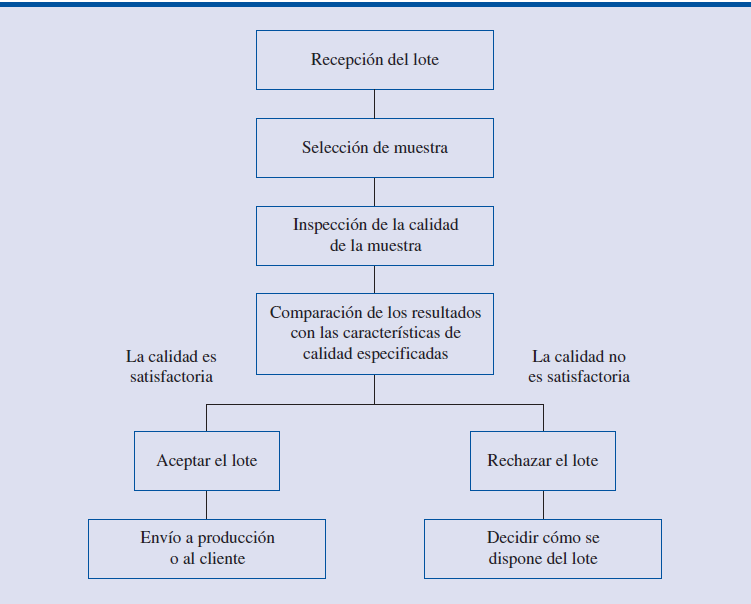
\includegraphics[width=9.5cm]{IMAGENES/MA.png}
        \label{figura1}
\end{figure}
\end{frame}

\begin{frame}
\frametitle{Marco Teórico}
\begin{block}{Marco estadístico}
~\\El muestreo de aceptación puede dividirse en dos tipos fundamentales dependiendo de la característica observada:
\begin{itemize}
\justifying
\item Muestreo por atributos: cuando en la inspección los artículos se dividen en defectuosos y en no defectuosos, según cumplan con un conjunto de requerimientos.
\item Muestreo por variables: cuando en la inspección se mide una variable cuantitativa: longitudes, pesos... y se evalúa la distancia entre dicha cantidad y la requerida en las especificaciones.
\end{itemize}
~\\En el muestreo de aceptación se utilizan principalmente tres distribuciones de probabilidad dependiendo del tamaño del lote(grande o pequeño), las distribuciones utilizadas son la Hipergeométrica, la Poisson y la Binomial.
\end{block}
\end{frame}

\begin{frame}
\frametitle{Marco Teórico}
\begin{block}{Marco estadístico}
\begin{itemize}
\justifying
\item Distribución hipergeométrica:La distribución hipergeométrica es fundamental para gran parte del muestreo de aceptación. Es aplicable cuando se muestrea una característica de atributo de un lote finito ó pequeño sin reemplazo. Su función de probabilidad es:
$$f(x)=\frac{\binom{N_p}{x}\binom{N_q}{n-x}}{\binom{N}{n}}$$
~\\ Donde; 
~\\ N es el tamaño del lote, $N>0$
~\\ p es la proporción defectuosa en el lote, $p=0, 1/N, 2/N, \cdots , 1$
~\\ q es la proporción efectiva en el lote, $q = 1 – p$
~\\ n es el tamaño de la muestra, $n = 1, 2, …, N$
~\\ x es el número de ocurrencias, $x = 0, 1, 2, …, n$
\end{itemize}
\end{block}
\end{frame}

\begin{frame}
\frametitle{Marco Teórico}
\begin{block}{Marco estadístico}
\begin{itemize}
\justifying
\item Distribución binomial: Es la distribución más utilizada en el muestreo de aceptación. Complementa la hipergeométrica en el sentido de que se emplea al muestrear una característica de atributo de un lote (o proceso) infinito ó grande, o un lote finito cuando se toma una muestra con reemplazo. Su función de probabilidad es:
$$f(x)=\binom{n}{x} \; p^x \; (1-p)^{n-x}=\binom{n}{x} \; p^x \; q^{n-x}$$
~\\ Donde; 
~\\ n es el tamaño de la muestra, $n>0$
~\\ p es la proporción defectuosa, $0\leq p \leq 1$
~\\ q es la proporción efectiva, $q = 1 – p$
~\\ x es el número de ocurrencias, $x = 0, 1, 2, …, n$
\end{itemize}
\end{block}
\end{frame}

\begin{frame}
\frametitle{Marco Teórico}
\begin{block}{Marco estadístico}
\begin{itemize}
\justifying
\item Distribución poisson: La distribución de Poisson se utiliza para calcular las características de los planes de muestreo, que especifican un número dado de defectos por unidad, como el número de remaches defectuosos en el ala de un avión o el número de piedras permitido en un pedazo de vidrio de un tamaño determinado. El parámetro en la distribución de Poisson es simplemente $\mu$. Su función de probabilidad es:
$$f(x)=\frac{{\mu}^x \; e^{-\mu}}{x!}$$
~\\ Donde; 
~\\ $\mu$ es el número medio de defectos, $\mu>0$
~\\ x es el número de ocurrencias, $x=0,1,2,\cdots$
\end{itemize}
\end{block}
\end{frame}

\begin{frame}
\frametitle{Marco Teórico}
\begin{block}{Marco estadístico}
\begin{itemize}
\justifying
\item Curva característica de operación: Es una representación gráfica del rendimiento de un plan de muestreo. Se crea trazando la probabilidad de que el lote sea detectado, para toda una gama de proporciones de unidades defectuosas. Esta gráfica describe el grado en que un plan de muestreo permite distinguir entre los lotes buenos y los lotes malos. \cite{OPE}

~\\En el muestreo de aceptación de lotes, se deben determinar ciertos parámetros que nos permitan decidir si rechazamos o aceptamos el lote a partir de los datos recogidos en la muestra, esos parámetros son:
\item Número de aceptación: Es el número de unidades infestadas o el número de plagas individuales permitidas en una
muestra de determinado tamaño, antes de que se tomen medidas fitosanitarias.\cite{MUES}
\end{itemize}
\end{block}
\end{frame}

\begin{frame}
\frametitle{Marco Teórico}
\begin{block}{Marco estadístico}
\begin{itemize}
\justifying
\item Nivel de detección:Es el porcentaje o la proporción de infestación mínimo que detectará la metodología de muestreo
al nivel de eficacia de detección y el nivel de confianza especificado.\cite{MUES}
\item Nivel de confianza:Indica la probabilidad de que un envío con un grado de infestación que exceda el nivel de
detección será detectado. Se suele utilizar un nivel de confianza del 95\%.\cite{MUES}
\item Eficacia de la detección: La eficacia de la detección es la probabilidad de que la inspección o la prueba de diagnóstico de una o más unidades
infestadas detectará una plaga. En general, no debería suponerse que habrá un 100\% de eficacia.\cite{MUES}
\item Tamaño de la muestra: Es la cantidad de unidades seleccionadas del lote o envío que se inspeccionarán o someterán a
pruebas de diagnóstico.\cite{MUES}
\item Nivel de tolerancia:Se refiere al porcentaje de infestación de todo el envío o lote que constituye el umbral para la acción fitosanitaria.En general, se utiliza un nivel de tolerancia 0.\cite{MUES}
\end{itemize}
\end{block}
\end{frame}

\section{Metodología}
\begin{frame}
\frametitle{Metodología}
\begin{block}{Propuesta}
\begin{itemize}
\item Definición del caso
\item Criterio de aceptación/rechazo
\item Enfermedades (asintomáticas – no asintomáticas)
\item Tipos de vivero (con regulaciones – sin regulaciones)
\item Tipo de muestreo
\item Simulación
\item Análisis y validación del muestreo
\end{itemize}
\end{block}
\end{frame}

\section{Cronograma}
\begin{frame}
\frametitle{Cronograma}
\Wider[4em]{
\begin{figure}[!h]
        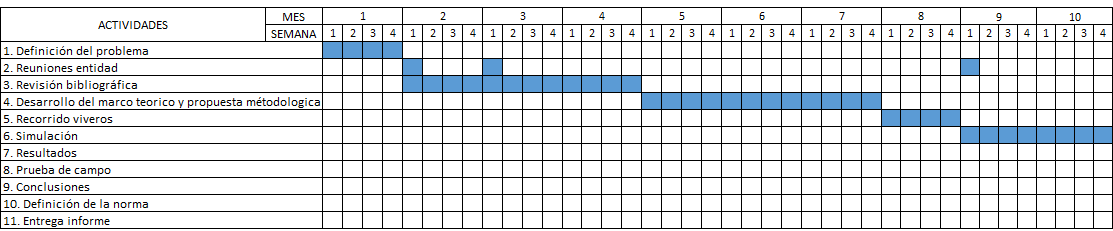
\includegraphics[width=12.4cm]{IMAGENES/CR1.png}
        \label{figura1}
\end{figure}
\begin{figure}[!h]
        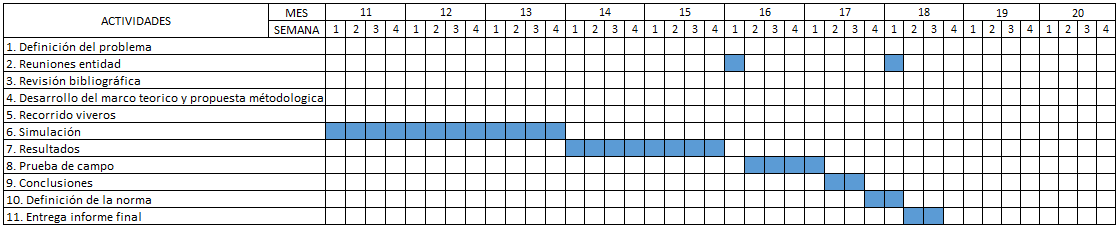
\includegraphics[width=12.4cm]{IMAGENES/CR2.png}
        \label{figura1}
\end{figure}

}
\end{frame}

\section{Presupuesto}
\begin{frame}
\frametitle{Presupuesto}
\begin{figure}[!h]
        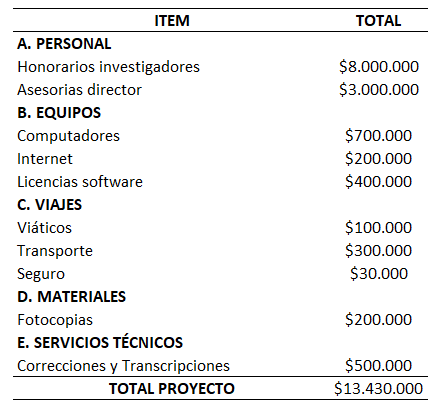
\includegraphics[width=8cm]{IMAGENES/PR.png}
        \label{figura1}
\end{figure}
\end{frame}



\bibliographystyle{plain}
  \bibliography{references}
\end{document}
